\chapter{Event reconstruction}

In this chapter the procedure for event reconstruction of the $B$ meson decay $B \to K K \ell \nu$ is shown, starting with final state particle selection and then combining them to obtain $B$ meson candidates.

\section{Final state particles selection}
Since the neutrino escapes detection, we can only reconstruct the charged tracks in the decay, which are the two charged kaons ($K$) and the light lepton, which is the electron ($e$) or muon ($\mu$). These are some of the particles which are commonly referred to as final state particles (FSP). Final state particles have a long lifetime and are usually the particles that we detect when they interact with the material in the detector.

It is important to limit our selection of FSP particles in order to cut down the number of particle combinations, and consequentially computation time and file sizes.

\subsubsection{Leptons}

Figures \ref{fig:evars} and \ref{fig:muvars} show the impact parameters $d_0$ and $z_0$, the momentum in  $\Upsilon(4S)$ center-of-mass system (CMS), and the PID information for true and fake electrons and muons, where an extra category for true electrons/muons from the signal decay is shown.

\begin{figure}[H]
\centering
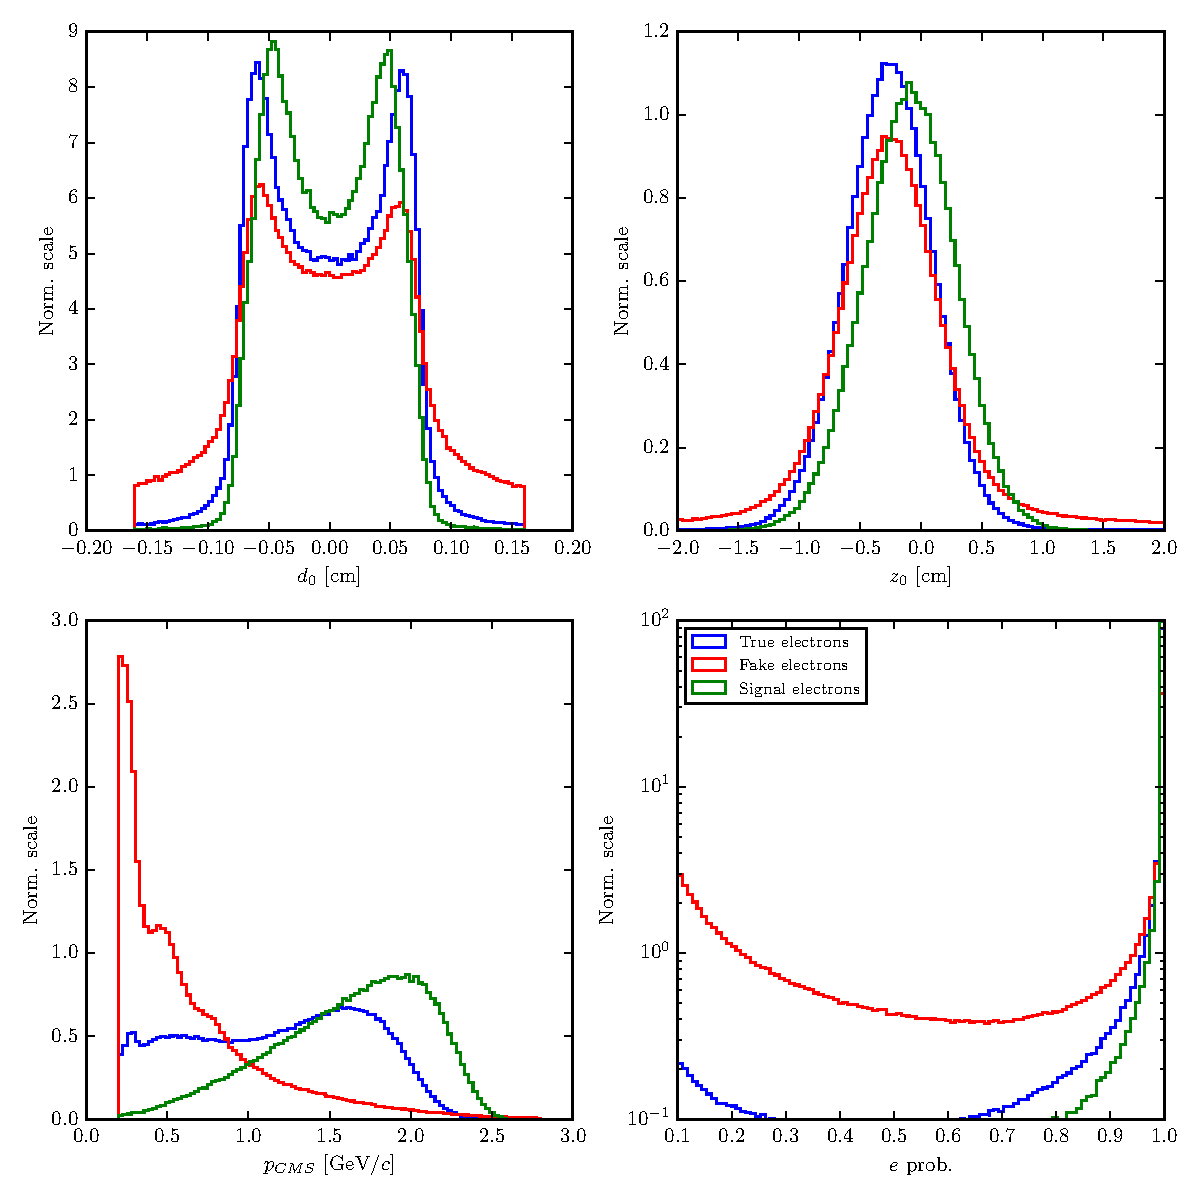
\includegraphics[width=\linewidth]{fig/FSP_e_vars}
\captionsetup{width=.8\linewidth}
\caption{Normalized properties of true (blue), fake (red) and true electrons from signal $B$ candidates (green).}
\label{fig:evars}
\end{figure}

\begin{figure}[H]
\centering
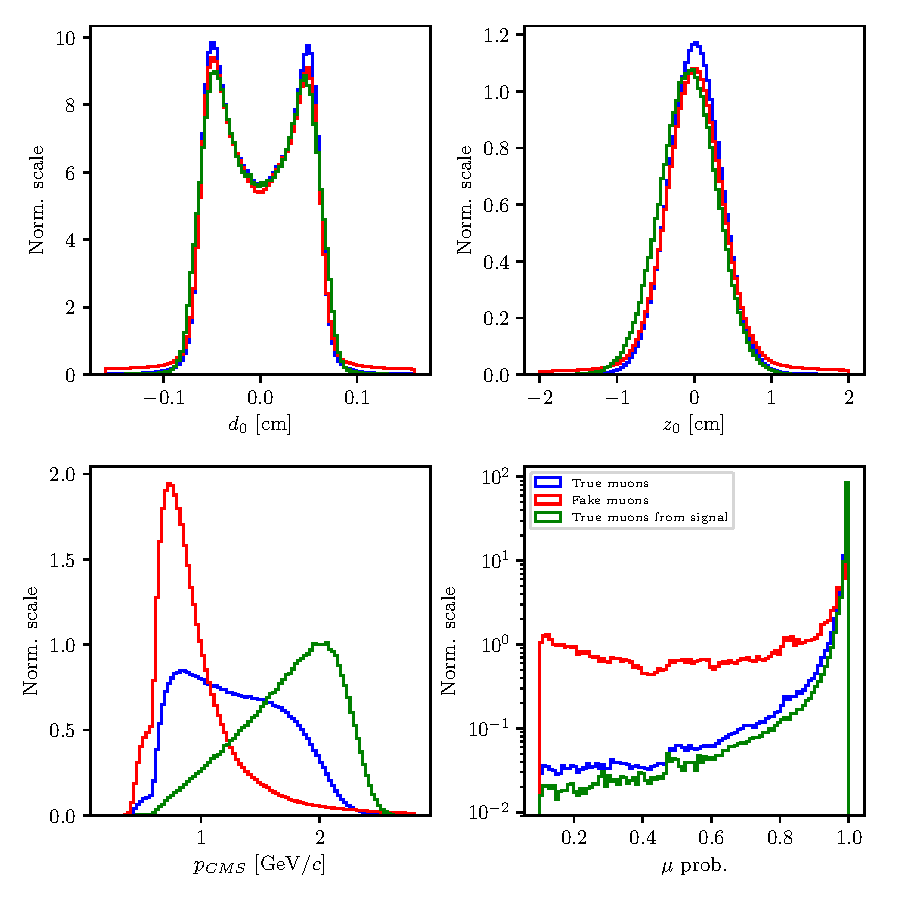
\includegraphics[width=\linewidth]{fig/FSP_mu_vars}
\captionsetup{width=.8\linewidth}
\caption{Normalized properties of true (blue), fake (red) and true muons from signal $B$ candidates (green).}
\label{fig:muvars}
\end{figure}

Based on these distributions, we can define a set of cuts
\begin{itemize}
\item $\vert d_0 \vert < 0.1\e{cm}$,
\item $\vert z_0 \vert < 1.5\e{cm}$,
\item $p_{CMS} \in [0.4,\,2.6]~\e{GeV}/c$ for electrons,
\item $p_{CMS} \in [0.6,\,2.6]~\e{GeV}/c$ for muons.
\end{itemize}

After this selection we can determine the optimal PID cuts for electrons and muons, where we optimize the selection by maximizing the standard definition of \textit{figure of merit} ($\mathrm{FOM}$), defined in Eq. (\ref{eq:fom})
\begin{equation}
\label{eq:fom}
\mathrm{FOM} = \sqrt{\mathcal{E}\mathcal{P}} \propto \frac{S}{\sqrt{S+B}},
\end{equation} 
where the argument in the square root is the product of the efficiency ($\mathcal{E}$) and the purity ($\mathcal{P}$) function. The definitions of signal ($S$) and background ($B$) are somewhat fluid throughout the analysis and need to be defined for each $\mathrm{FOM}$ separately. In this section we define two representations of $S$ and $B$. In $\mathrm{FOM}_1$ the signal $S$ represents correctly reconstructed final state particles, while in $\mathrm{FOM}_2$ the signal $S$ represents correctly reconstructed final state particles which also come from a correctly reconstructed $B$ meson candidate. In both cases $B$ represents all other particle candidates which do not satisfy the conditions of $S$.

The $\mathrm{FOM}$ plots are shown in Figures \ref{fig:efom} and \ref{fig:mufom}. The cut values are based on PID cuts used for PID efficiency calibration. The optimal value for the PID cuts is equal to the largest available value, regardless of the leptons coming from signal decays or not. The optimized PID cuts for leptons are
\begin{itemize}
\item $e$ prob. $ > 0.9$ for electrons,
\item $\mu$ prob. $ > 0.97$ for muons.
\end{itemize}

\begin{figure}[H]
\centering
\captionsetup{width=.8\linewidth}
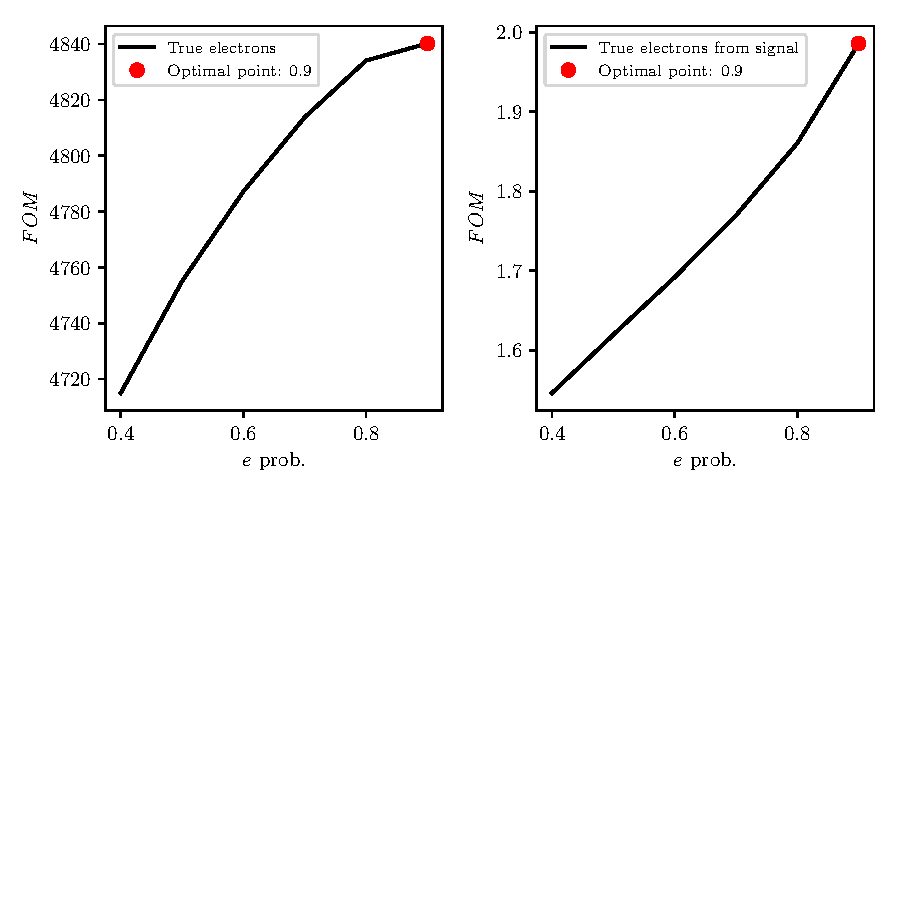
\includegraphics[width=\linewidth]{fig/FSP_e_fom}
\caption{$\mathrm{FOM}$ optimizations of the PID probability cuts for true electrons (left) and true electrons from signal $B$ candidatess (right).}
\label{fig:efom}
\end{figure}

\begin{figure}[H]
\centering
\captionsetup{width=.8\linewidth}
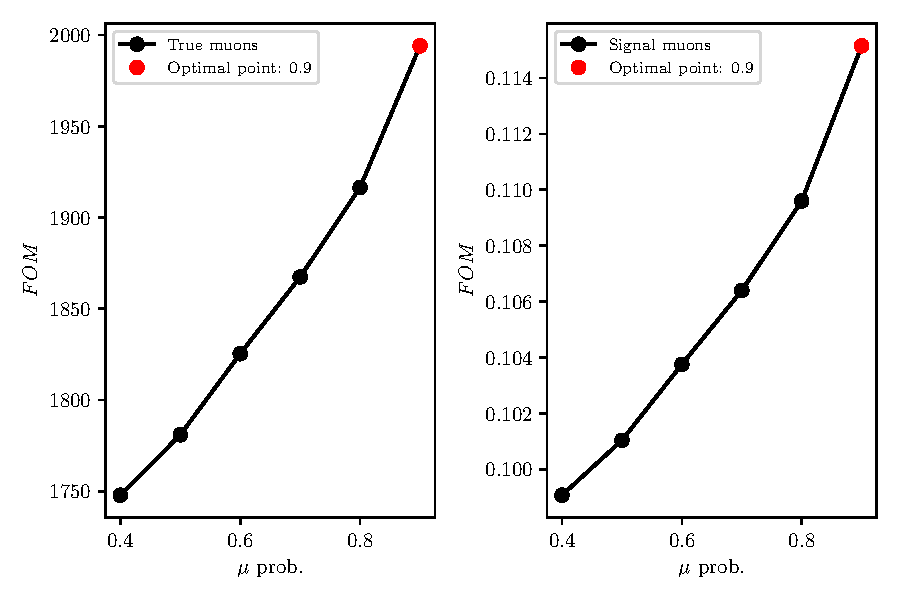
\includegraphics[width=\linewidth]{fig/FSP_mu_fom}
\caption{$\mathrm{FOM}$ optimizations of the PID probability cuts for true muons (left) and true muons from signal $B$ candidates (right).}
\label{fig:mufom}
\end{figure}


\subsubsection{Kaons}

We repeat the procedure for both kaons. Figure \ref{fig:Kvars} shows the impact parameters $d_0$ and $z_0$, the momentum in  $\Upsilon(4S)$ center-of-mass system (CMS), and the PID information for true and fake kaons, where an extra category for true kaons from the signal decay is shown.

\begin{figure}[H]
\centering
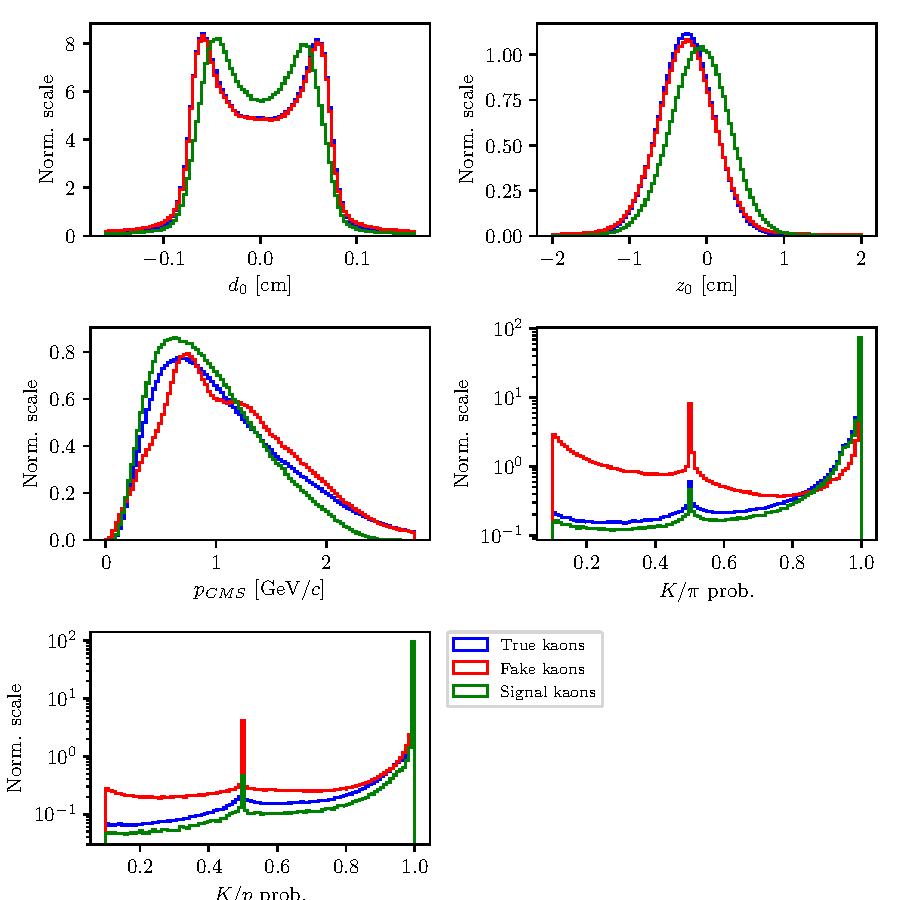
\includegraphics[width=\linewidth]{fig/FSP_kaon_vars}
\captionsetup{width=.8\linewidth}
\caption{Normalized properties of true (blue), fake (red) and true kaons (green) from signal $B$ candidates.}
\label{fig:Kvars}
\end{figure}

We define the kaon cuts in the same manner as in the case for leptons
\begin{itemize}
\item $\vert d_0 \vert < 0.15\e{cm}$,
\item $\vert z_0 \vert < 1.5\e{cm}$,
\item $p_{CMS} \in [0,\,2.5]~\e{GeV}/c$.
\end{itemize}

The PID optimization in this case is taken in two steps. First we optimize the cut on $K / \pi$, and after that the $K/p$ separation probability. Figure \ref{fig:Kfom} shows the optimization procedure for PID cuts on kaon candidates.

\begin{figure}[H]
\centering
\captionsetup{width=.8\linewidth}
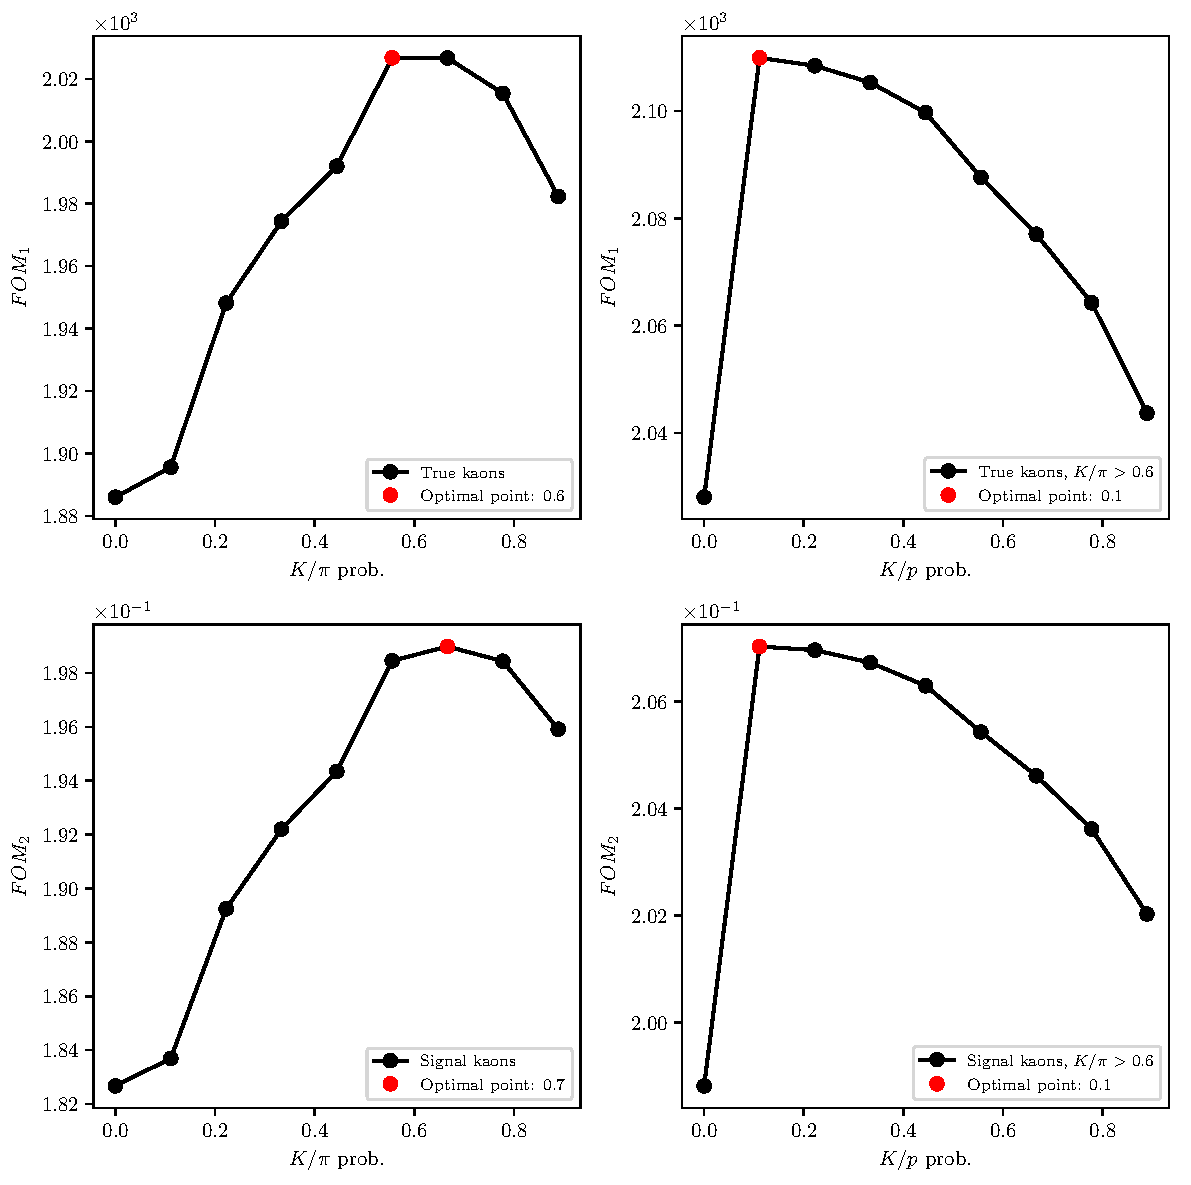
\includegraphics[width=\linewidth]{fig/FSP_kaon_fom}
\caption{$\mathrm{FOM}$ optimizations of the PID probability cuts for true kaons (top) and true kaons from signal $B$ candidates (bottom). The plots on the left show the optimization of the first step for the $K / \pi$ probability cut, and the plot on the right the $K/p$ probability cut.}
\label{fig:Kfom}
\end{figure}

The optimized PID cuts for kaons are
\begin{itemize}
\item $K/\pi > 0.6$,
\item $K/p > 0.1$.
\end{itemize}

\section{Combination of FSP particles}

With the pre-selected kaon and lepton candidates we make combinations for potential $B$ meson candidates. Since the missing neutrino escapes detection, we reconstruct the $B$ mesons in the following two channels
\begin{align*}
B^+ &\to K^+ K^- e^+, \\
B^+ &\to K^+ K^- \mu^+,
\end{align*}
and similarly for $B^-$. When an arbitrary combination is obtained, we perform a vertex fit of the three tracks in order to discard combinations with a low probability of tracks coming from the same point. $B$ mesons have a relatively long lifetime and decay along the $z$ axis of the detector in the direction of the boost, so the vertex fit is enforced with an \texttt{IPTUBE} constraint, which constrains the vertex to an elongated ellipsoid along beam direction. We demand that the fit converged and apply a cut on the minimal fit probability. The fit probability for signal and background $B$ meson candidates is shown in Figure \ref{fig:vtx} (left). We perform a $\mathrm{FOM}$ cut optimization of this variable, which is shown in Figure \ref{fig:vtx} (right). In this and in the following cases, the definition of $S$ from Eq. (\ref{eq:fom}) are correctly reconstructed $B$ meson candidates with a missing neutrino which are not coming from the $b \to c$ transition.

\begin{figure}[H]
\centering
\captionsetup{width=0.8\linewidth}
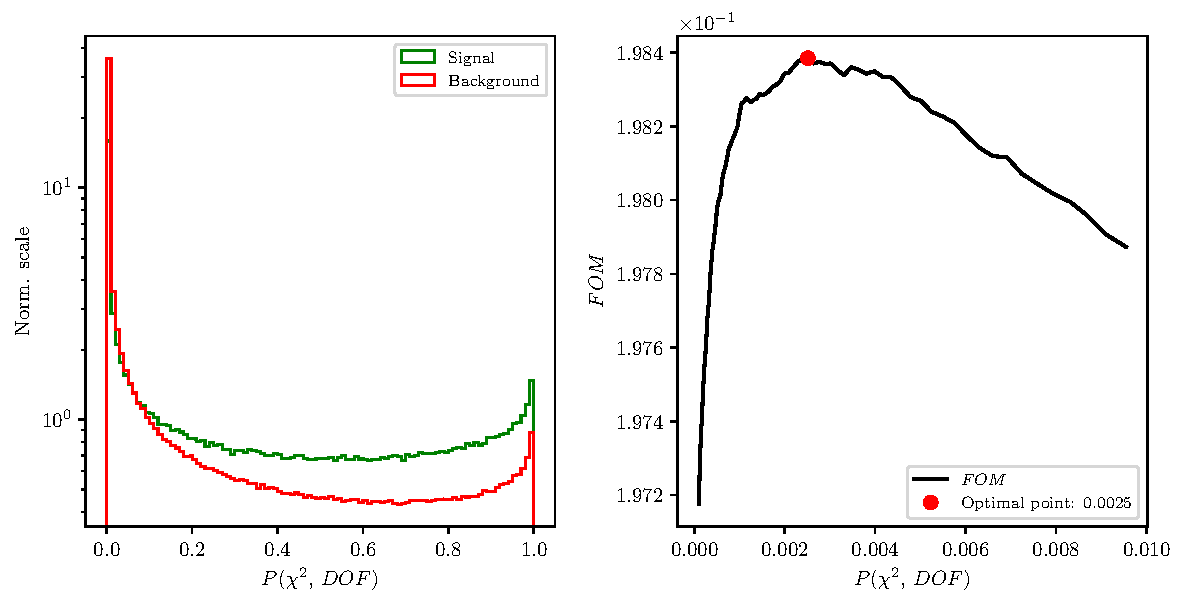
\includegraphics[width=\linewidth]{fig/VTX}
\caption{Normalized vertex fit probability distribution for signal and background $B$ meson candidates in logarithmic scale (left) and $\mathrm{FOM}$ optimization of the vertex fit probability (right).}
\label{fig:vtx}
\end{figure}

Even though the vertex fit probability cut was optimized, we choose a slightly different but a more standard cut of
\begin{itemize}
\item $P(\chi^2,NDF) > 1.0\E{-3}$.
\end{itemize}

With the neutrino being the only missing particle on the reconstructed side, it is possible to determine the angle between the direction of the reconstructed $B$ (denoted as $Y \to K K \ell$) and the nominal $B$, as
\begin{align}
\mathrm{p}_\nu &= \mathrm{p}_B - \mathrm{p}_{Y}, \\
\label{eq:massnu}
\mathrm{p}_\nu^2 = m_\nu^2 &= m_B^2 + m_Y^2 - 2E_BE_Y + 2\vec{p}_B \cdot \vec{p}_Y \approx 0, \\ 
\label{eq:cosby}
\cos \left(\theta_{BY}\right) &= \frac{2E_BE_Y - m_B^2 - m_Y^2}{2\vert \vec{p}_B \vert \vert \vec{p}_Y\vert},
\end{align} 

where all the energy and momenta above are calculated in the CMS frame. The mass of the neutrino is equal to 0 to a very good precision, so we use it in Eq. (\ref{eq:massnu}). In addition, we can substitute the unknown energy and momentum magnitude, $E_B$ and $\vert \vec{p}_B \vert$, of the $B$ meson in Eq. (\ref{eq:cosby}), with quantities from the well known initial conditions
\begin{align}
E_B &= E_{CMS} / 2,\\
\vert \vec{p}_B \vert = p_B &= \sqrt{E_B^2 - m_B^2},
\end{align} 

where $E_{CMS}$ is the total energy of the $e^+e^-$ collision in the CMS frame and $m_B$ is the nominal mass of the $B$ meson. 

For the correctly reconstructed candidates, this variable lies in the $[-1,1]$ region, though only to a certain precision, due to the finite detector resolution. For background candidates, however, the candidates populate also the non-physical regions, as shown in Figure \ref{fig:cosby} (left). We impose an optimized cut on this variable from Figure \ref{fig:cosby} (right) to discard a large amount of background.
\begin{itemize}
\item $\vert \cos \left(\theta_{BY}\right) \vert < 1.0$.
\end{itemize}

\begin{figure}[H]
\centering
\captionsetup{width=.8\linewidth}
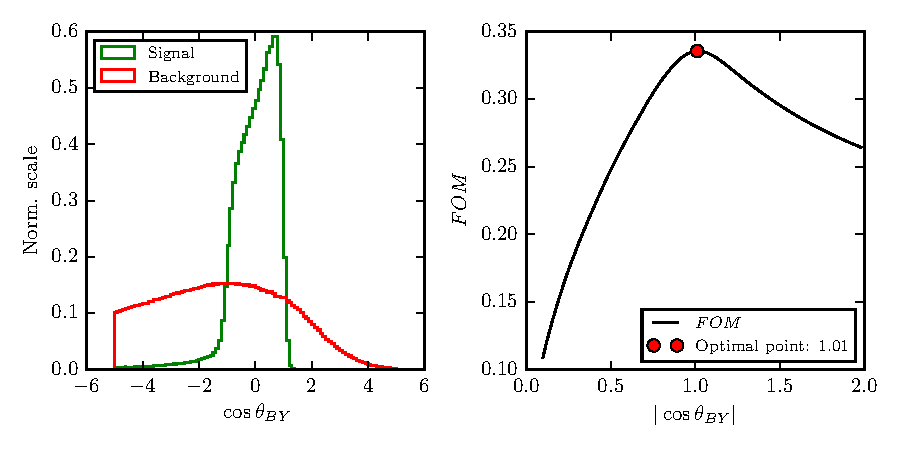
\includegraphics[width=\linewidth]{fig/cosBY}
\caption{Normalized $\cos \theta_{BY}$ distribution for signal and background $B$ meson candidates (left) and $\mathrm{FOM}$ optimization of the $\cos \theta_{BY}$ variable (right).}
\label{fig:cosby}
\end{figure}

\section{Loose neutrino reconstruction}\label{sec:loose-neutrino-reconstruction}

%Due to the beam background in the detector, material interactions, or other processes, random tracks and clusters enter our event and get reconstructed as part of the physics process we want to study. These tracks and clusters are not interesting and further spoil the data we measure. In order to remedy this, we perform an extensive clean-up of the tracks and clusters in the ROE side before calculating the four-momentum of the missing part of the event. The clean-up procedure is performed separately on tracks and clusters and uses multiple steps with multivariate analysis (MVA) algorithms in order to separate good tracks and clusters from the bad ones, which populate the ROE. Then, for each ROE object, a ROE mask is created for tracks and clusters, which narrates the use of this track or cluster in the final calculations of the ROE four-momentum.
%
%In order to preserve the continuity of this chapter, a more detailed description of the ROE clean-up can be found in Chapter \ref{ch:roe}. From this point on we assume the ROE to be efficiently cleansed of extra tracks and clusters .


The signal-side neutrino escapes detection, so we cannot directly determine it's four-momentum. However, due to the detectors geometry, which almost completely covers the full solid angle, and due to well known initial conditions of the $\Upsilon(4S)$ meson, it is possible to determine the kinematics of the missing neutrino via indirectly reconstructing the companion $B$ meson by summing up the four-momenta of all the FSP particles in the event which were not used in the reconstruction of the signal side $B$ meson. This is known as the \textit{untagged} method since we are not using any kind of tagging method to reconstruct the companion $B$ meson. The particles used in the indirect companion $B$ meson reconstruction are also said to belong to the \textit{rest of the event} (ROE).

Due to the beam background in the detector, material interactions, or other processes, random tracks and clusters enter our event and get reconstructed as part of the physics process we want to study. These tracks and clusters are not interesting and further spoil the data we measure. In order to remedy this, we perform an extensive clean-up of the tracks and clusters in the ROE side before calculating the four-momentum of the missing part of the event. Here we see the motivation for the ROE clean-up, since our signal candidate reconstruction depends on tracks and clusters in the ROE side. The clean-up procedure is performed separately on tracks and clusters and uses multiple steps with multivariate analysis (MVA) algorithms in order to separate good tracks and clusters from the bad ones, which populate the ROE. Then, for each ROE object, a ROE mask is created for tracks and clusters, which narrates the use of this object in the final calculations of the ROE four-momentum. From this point on we assume the ROE to be efficiently cleansed of extra tracks and clusters. A more detailed description of the ROE clean-up can be found in Chapter \ref{ch:roe}. 

The total missing four-momentum in the event can be determined as
\begin{align}
\mathrm{p}_{miss} &= \mathrm{p}_{\Upsilon(4S)} - \sum_i^{\mathrm{Event}}\left(E_i,\,\vec{p}_i \right),\\
\label{eq:ROEloop}
\mathrm{p}_{miss} &= \mathrm{p}_{\Upsilon(4S)} - \left(\mathrm{p}_{Y} -\sum_i^{\mathrm{Rest~of~event}}\left(E_i,\,\vec{p}_i \right)\right),
\end{align}

where the summation runs over all charged and neutral particles in the defined set with
\begin{equation}
\mathrm{p}^{neutral}_i = \left(p_i,\, \vec{p}_i \right) \quad \mathrm{and} \quad \mathrm{p}^{charged}_i = \left(\sqrt{m_i^2 + p_i^2},\, \vec{p}_i \right),
\label{eq:pcharged}
\end{equation}
where we assumed all neutral particles to be massless photons. For charged tracks in the ROE a mass hypothesis needs to be defined in order to determine the track's energy. After the ROE clean-up we make the following procedure of choosing the mass hypothesis
\begin{enumerate}
\item $e$, if $e$ prob. $> \mu$ prob. and $e$ prob. $> 0.9$,
\item otherwise $\mu$, if $\mu$ prob. $> e$ prob. and $\mu$ prob. $> 0.97$,
\item otherwise $K$, if $K/\pi$ prob. $> 0.6$,
\item otherwise $\pi$.
\end{enumerate} 
We define the square of the missing mass, $m_{miss}^2$, which is consistent with zero, if signal-side neutrino is the only missing particle in the event, as shown in Eq. (\ref{eq:m2def}).
\begin{align}
\label{eq:nuold}
\mathrm{p}_\nu &= \mathrm{p}_{miss} = \left(E_{miss},\,\vec{p}_{miss} \right),\\
\label{eq:m2def}
m_{miss}^2 &= \mathrm{p}_{miss}^2 = \mathrm{p}_{\nu}^2 = m_\nu^2 \approx 0.
\end{align}

Since the detector is not perfect, the distribution of the $m_{miss}^2$ variable has a non-zero width. Additionally, tails are introduced as soon as we have missing particles such as extra missing neutrinos, other neutral undetected particles such as $K_L^0$, or simply missing tracks due to detection failure. Figure \ref{fig:missm2} shows the distribution of $m_{miss}^2$ as defined with the missing four-momentum in Eq. (\ref{eq:nuold}). Correctly reconstructed candidates, which come from events where the other $B$ meson decayed via a hadronic decay mode, should peak at zero. If this is not the case, candidates are shifted to larger values of this variable. Due to this fact, we impose a cut on the $m_{miss}^2$ variable in order to partially discard candidates with spoiled properties, even if it was in principle a correct combination of FSP particles on the signal side
\begin{itemize}
\item $\vert m_{miss}^2 \vert < 7\e{GeV}/c^2$.
\end{itemize}

For further purposes in this analysis we also define a subset of all signal candidates, which come from events where the companion $B$ meson decayed hadronically and all of it's particles were taken into account correctly. We only allow for missing photons, since they are frequently irradiated due to brehmsstrahlung effects and don't have such a big impact on the 4-momentum of the final candidate. We denote this subset as \textit{perfect} signal.

This cut on $m_{miss}^2$ was not optimized as the optimal case would result in a too strong threshold if optimized on perfect signal sample, since we still may want to retain as much signal candidates as possible, even if they are coming from events with semi-leptonic decays of the other $B$ meson.

\begin{figure}[H]
\centering
\captionsetup{width=.8\linewidth}
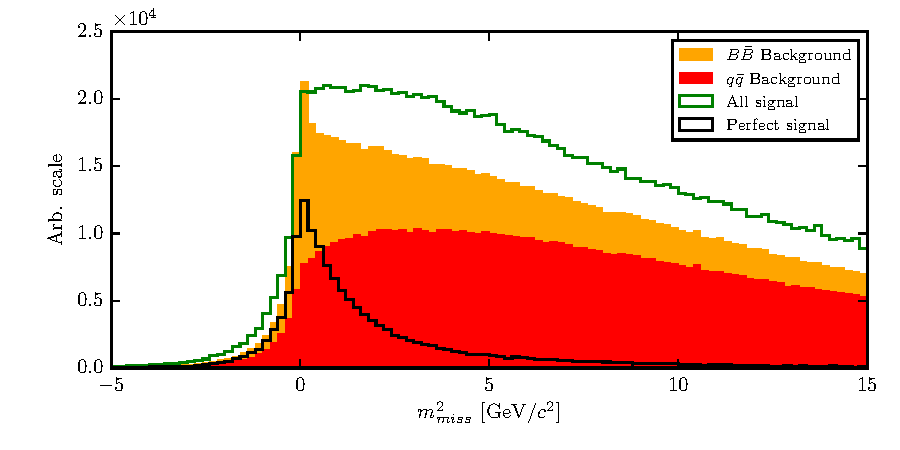
\includegraphics[width=\linewidth]{fig/missM2}
\caption{Squared missing mass distribution for $q \bar q$ and $B \bar B$ background in filled histograms. All signal (green) and perfect signal (black) are scaled up equally.}
\label{fig:missm2}
\end{figure}

The main uncertainty of the neutrino four-momentum, defined in Eq. (\ref{eq:nuold}), comes from energy uncertainty. It is a common practice to substitute the missing energy with the magnitude of the missing momentum, since the momentum resolution from the measurement is much better, thus redefining the neutrino four-momentum to
\begin{equation}
\label{eq:nunew}
\mathrm{p}_\nu = \left(\vert \vec{p}_{miss} \vert,\,\vec{p}_{miss} \right),
\end{equation}
which fixes the neutrino mass to $0\e{GeV}/c^2$.

The newly defined neutrino four-momentum can be added to the four-momentum of the $Y(KK\ell)$ candidate to obtain the full $B$ meson four-momentum and calculate the traditional $M_{BC}$ and $\Delta E$ variables
\begin{align}
\label{eq:de}
\Delta E &= E_B - E_{CMS}/2,\\
M_{BC} &= \sqrt{\left(E_{CMS}/2\right)^2 - \vert \vec{p} \vert^2}.
\end{align}

Since the final fit will be performed over \vars, we define the fit region
\begin{itemize}
\item $M_{BC} \in [5.1,\,5.295]\e{GeV}/c^2$,
\item $\Delta E \in [-1.0,\,1.3]\e{GeV}$.
%\item Signal enhanced region: $M_{BC} \in [5.27,\,5.295]\e{GeV}/c^2$ and $\vert \Delta E \vert < 0.143 \e{GeV}$,
\end{itemize}

Figure \ref{fig:mbc_de_pre} shows the distributions of $\Delta E$ (left) and $M_{BC}$ (right) for signal and major types of background after the pre-cuts. Both signal components are scaled up with respect to the background components, but are in proper scale one to another. The effects of missing particles are clearly seen based on the shape difference between all and perfect signal.

\begin{figure}[H]
\centering
\captionsetup{width=0.8\linewidth}
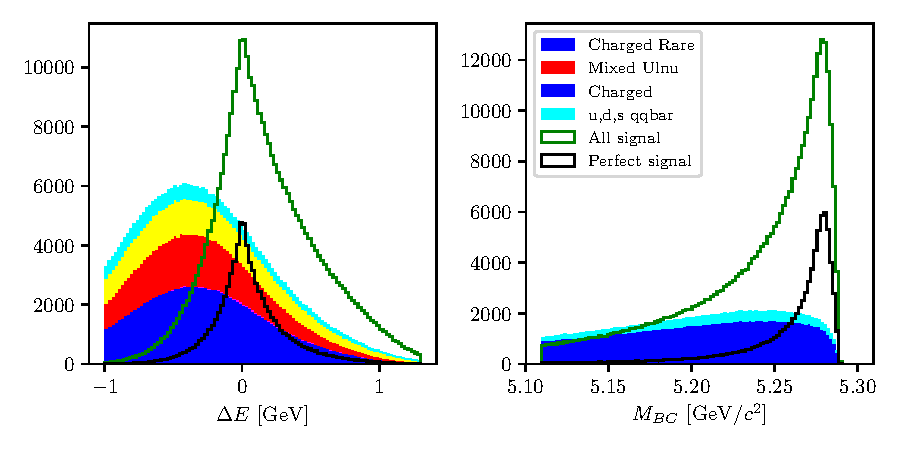
\includegraphics[width=\linewidth]{fig/mbc_de_pre}
\caption{Distributions of $\Delta E$ (left) and $M_{BC}$ (right) for signal and major types of background after the precuts. Both signal components are scaled up with respect to the background components, but are in proper scale one to another. The perfect signal has a much better resolution in both distributions, since the event is perfectly reconstructed.}
\label{fig:mbc_de_pre}
\end{figure}


%\section{$q^2$ calculation}
%
%Momentum transfer squared, $q^2$, is the squared Lorentz invariant of the four-momentum which is transferred from the $B$ meson to the $W$ boson. There are several possible calculations of this variable which offer different resolution. The following describes the calculation of $q^2$ which follows the calculation from [] and yields the best resolution.
%
%For correctly reconstructed events Eq. (\ref{eq:de}) satisfies the condition $\Delta E \approx 0$ within precision. It is possible to rescale the neutrino energy in such way that we fix $\Delta E$ to zero, meaning 
%\begin{equation}
%\Delta E' = (E_Y + \alpha E_\nu) - E_{CMS}/2 = 0.
%\end{equation}
%and calculate and adapted version of $M_{BC}$
%\begin{equation}
%M_{BC}' = \sqrt{\left(E_{CMS}/2\right)^2 - \vert \vec{p}_Y + \alpha \vec{p}_\nu \vert^2}.
%\end{equation}
%
%The neutrino momentum resolution dominates the $\Delta E$ uncertainty [], so the correction factor $\alpha$ reduces this source of uncertainty.
%
%A second correction can be applied by rotating the direction of the neutrino momentum by a small angle with respect to the reconstructed one. Such an angle is chosen in order fix the value of $M_{BC}'$ to the nominal mass of the $B$ meson, $m_B$.
%
%The corrected neutrino momentum is then solely used for the $q^2$ calculation, alongside the reconstructed lepton four-momentum, as
%\begin{equation}
%\label{eq:q2}
%q^2 = \mathrm{q}^2 = \left(\mathrm{p}_\ell + \mathrm{p}_\nu \right)^2.
%\end{equation}
%
%The $q^2$ distribution and its resolution are shown in Figure \ref{fig:q2}, along with additional versions of $q^2$, with details of the calculation method in the caption.
%\begin{figure}[H]
%\centering
%\captionsetup{width=0.8\linewidth}
%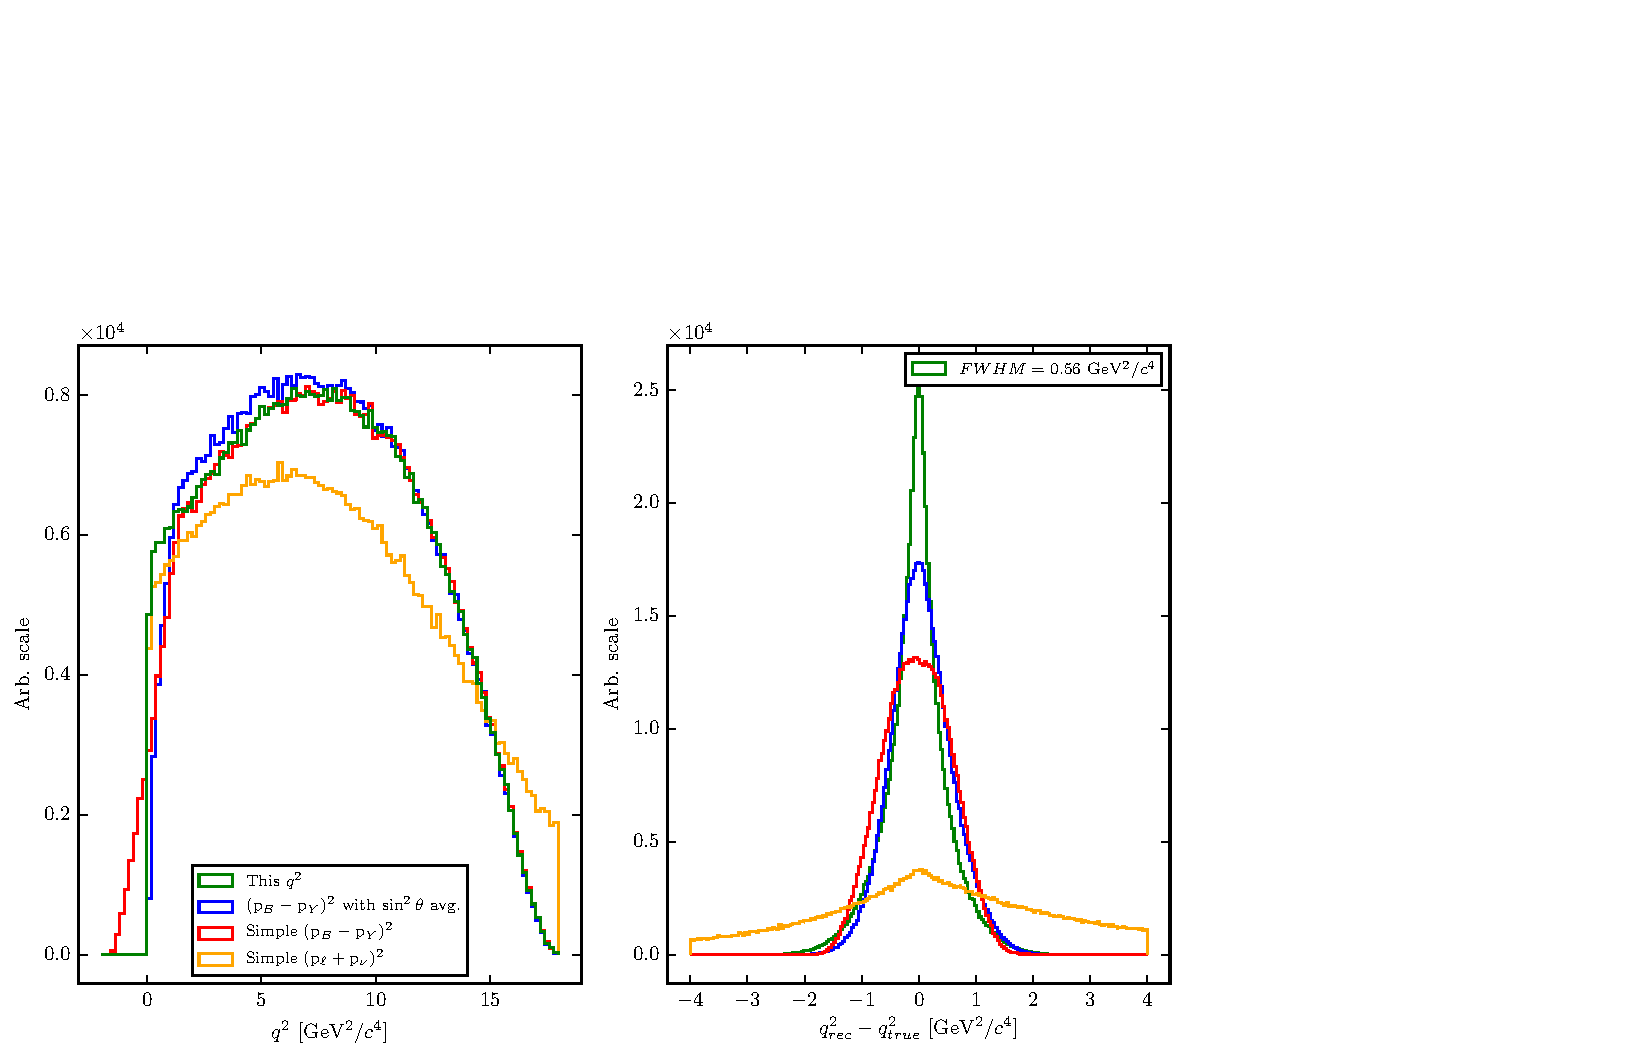
\includegraphics[width=\linewidth]{fig/q2}
%\caption{Distributions of $q^2$ (left) and $q^2$ resolution (right) for various methods of $q^2$ calculation. The blue distribution follows the procedure in [], whereas the red and the orange ones are straight-forward calculations with available information in the reconstruction. The $q^2$ calculation in red assumes a resting $B$ meson in the CMS frame, and the calculation in orange uses the neutrino four-momentum from Eq. (\ref{eq:nuold}).}
%\label{fig:q2}
%\end{figure}
%
%One must bare in mind that even though this calculation yields a precise result, this says nothing about the correctness of the $q^2$ model which was used (ISGW2) []. Since this decay has not been observed yet, we do not have a good description of the decay model, which is also a source of systematics in this analysis.

\section{Event categorization}\label{sec:event-categorization}

The missing information due to an escaping neutrino in our reconstructed channel is replaced by information from the companion $B$ meson. Since this is an untagged reconstruction, the quality of the companion $B$ meson affects the properties of signal candidate. Perfect reconstruction of a hadronically decayed companion $B$ meson results in pronounced peaks at $\Delta E \approx 0$, $m_{miss}^2 \approx 0$ and $M_{BC} \approx m_B$, while imperfect reconstruction due to any kind of missing particles produces long tails and/or a shift from the desired value in the mentioned distributions. These effects are undesired, since they make it harder to separate signal from background.

To remedy this, we split our signal candidates into 4 categories and work only with the best category. For categorization we use splitting in two ways. First, we look at the charge product of the reconstructed $B$ meson and the ROE object. For correctly reconstructed events, this should have a value of 
\begin{equation}
\label{eq:chargeprod}
q_{B^\pm}q_{B^\mp} = -1,
\end{equation}

however, this value is distributed due to missing charged particles in the reconstruction. Secondly, we train an MVA classifier based on ROE object properties in order to recognize companion $B$ mesons, which decayed hadronically. The details of the training are described in subsection \ref{subs:HDMVA} and in Addendum section \ref{sec:hadronic-decay-mva-training}.

We define 4 categories in the following way
\begin{enumerate} 
\item[]category I: $q_{B^\pm}q_{B^\mp} = -1$ and $BDT_{had.} > 0.51$,
\item[]category II: $q_{B^\pm}q_{B^\mp} \neq -1$ and $BDT_{had.} > 0.51$,
\item[]category III: $q_{B^\pm}q_{B^\mp} = -1$ and $BDT_{had.} \leq 0.51$,
\item[]category IV: $q_{B^\pm}q_{B^\mp} \neq -1$ and $BDT_{had.} \leq 0.51$,
\end{enumerate}

with the relative ratios of $37.74~\%$, $40.50~\%$, $13.43~\%$ and $8.32~\%$ for categories I, II, III and IV, respectively. Different categories for all signal candidates after the pre-cuts are shown in Figure \ref{fig:sig_categ}. Category I and II represent the majority of the candidates more or less equally, but category I has the best resolution, so we focus on candidates from category I in this analysis.

\begin{figure}[H]
\centering
\captionsetup{width=0.8\linewidth}
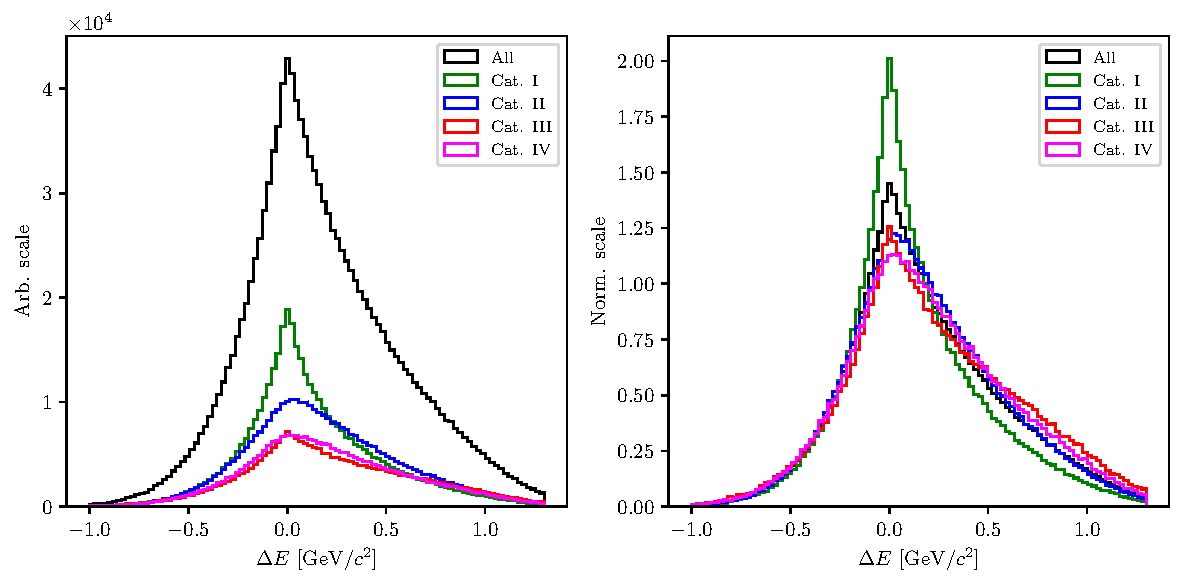
\includegraphics[width=\linewidth]{fig/sig_categ}
\caption{Categorization of signal candidates based on the charge product of both $B$ mesons in the event and the MVA output for recognizing hadronic decays of the companion $B$ meson. The plot on the left shows the distributions in an arbitrary scales, while the plot on the right shows the normalized distributions.}
\label{fig:sig_categ}
\end{figure}


\subsection{Hadronic decay MVA training}
\label{subs:HDMVA}

The Fast-BDT (FBDT) \cite{keck2017fastbdt} algorithm was used as the MVA classifier in all the following cases in this analysis. The following hyper-parameters were chosen for optimization
\begin{itemize}
\item \texttt{nTrees}: the number of trees in the FBDT forest,
\item \texttt{nLevels}: the number of levels in each FBDT tree.
\end{itemize}

Figure \ref{fig:BDT} shows a graphical interpretation of the FBDT forest with \texttt{nTrees} and \texttt{nLevels}. In all cases the hyper-parameters were optimized with a grid-search method in the hyper-parameter phase-space. 
\begin{figure}[H]
\centering
\captionsetup{width=0.8\linewidth}
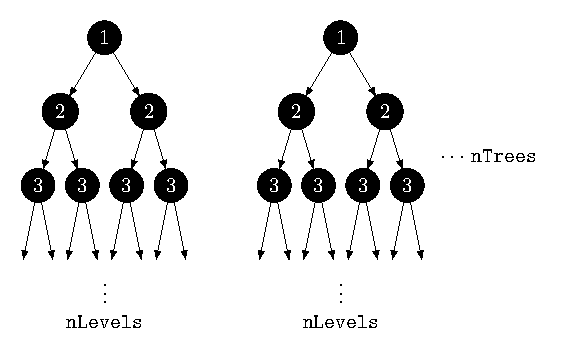
\includegraphics[scale=1]{texfig/BDT_forest}
\caption{A schematic of a BDT forest with \texttt{nTrees}, each tree having a depth of \texttt{nLevels}.}
\label{fig:BDT}
\end{figure}

In order to train an MVA classifier to recognize events with hadronically decaying $B$ mesons in the ROE side, we prepare a dataset of $2\E5$ candidates, where $50~\%$ of the candidates are signal $B$ candidates with hadronic decay of the companion $B$ meson. The remaining part of the training dataset consists of signal $B$ candidates with semi-leptonic decays of $B_{comp}$ and background $B$ candidates with hadronic and semi-leptonic decays of $B_{comp}$ in proportions $2:1:1$. 

The input variables used in this MVA are ROE specific and do not depend on the signal side. They are
\begin{itemize}
\item angle between tracks,
\item track quantities
	\begin{itemize}
	\item $P(\chi^2,DOF)$ of the tracks fit from the ROE side,
	\item $K$ and $\ell$ FlavorTagger variables,
	\item Charge of the ROE,
	\item $\cos \theta$ of the ROE momentum in the CMS frame,
	\item Number of tracks in ROE,
	\item Number of distant tracks in ROE, which don't pass requirements from Section \ref{s:ss}.
	\end{itemize}
\end{itemize}
%
The classifier output is shown in Figure \ref{fig:hdmva} (left). Candidates which populate the region with low values of the classifier output are more likely to come from semi-leptonic decays, so we want to discard those candidates. When optimizing the $\mathrm{FOM}$, we redefine the $S$ in Eq. (\ref{eq:fom}) to a correctly reconstructed signal candidate with a hadronically decayed companion $B$ meson. This $\mathrm{FOM}$ optimization, shown in Figure \ref{fig:hdmva} (right), yields the optimal cut
\begin{itemize}
\item $BDT_{had.} > 0.51.$
\end{itemize} 

\begin{figure}[H]
\centering
\captionsetup{width=0.8\linewidth}
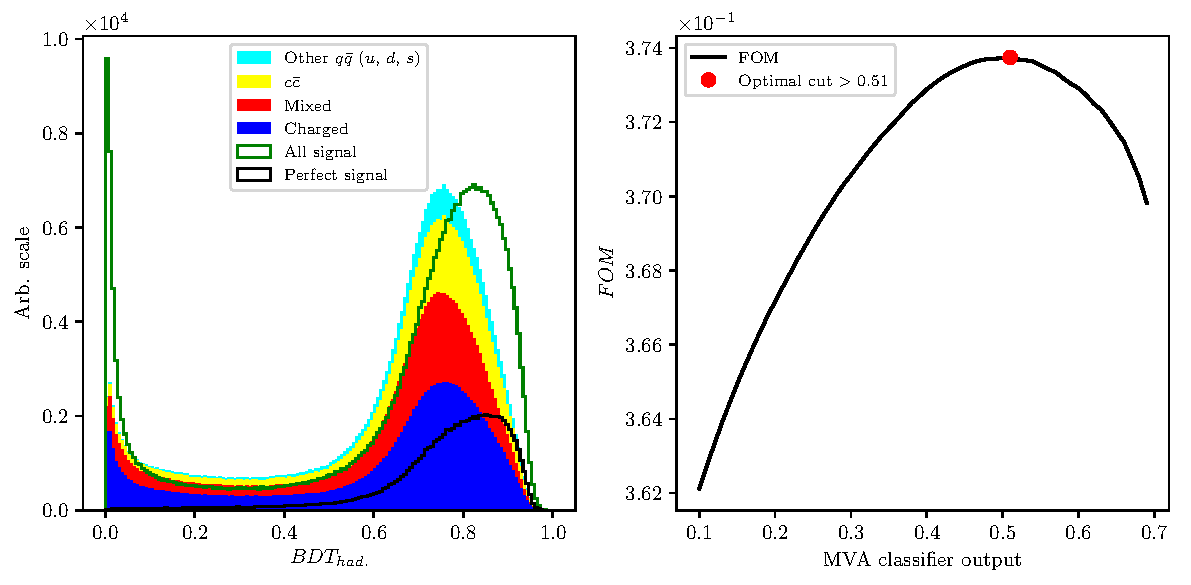
\includegraphics[width=\linewidth]{fig/hdmva_opt}
\caption{Hadronic MVA classifier output for major types of background and scaled-up signal (left), and $\mathrm{FOM}$ optimization on this cut for correctly reconstructed signal candidates with hadronically decayed companion $B$ meson (right).}
\label{fig:hdmva}
\end{figure}

More details on the hadronic MVA classifier training can be found in Appendix A.

\section{Signal region definition}

Since signal candidates are now categorized, we can define a signal region, where most of our perfectly reconstructed candidates lie. We use this region for optimizations of all cuts in the following steps of background suppression in chapter \ref{sec:background-suppression}. The 2D $\mathrm{FOM}$ optimization of the optimal $M_{BC}$ and $\Delta E$ is shown in Figure \ref{fig:sigwin}.
The signal region is defined as
\begin{itemize}
\item $M_{BC} > 5.270\e{GeV}/c^2.$,
\item $\vert \Delta E \vert < 0.166\e{Gev}$. 
\end{itemize}

\begin{figure}[H]
\centering
\captionsetup{width=0.8\linewidth}
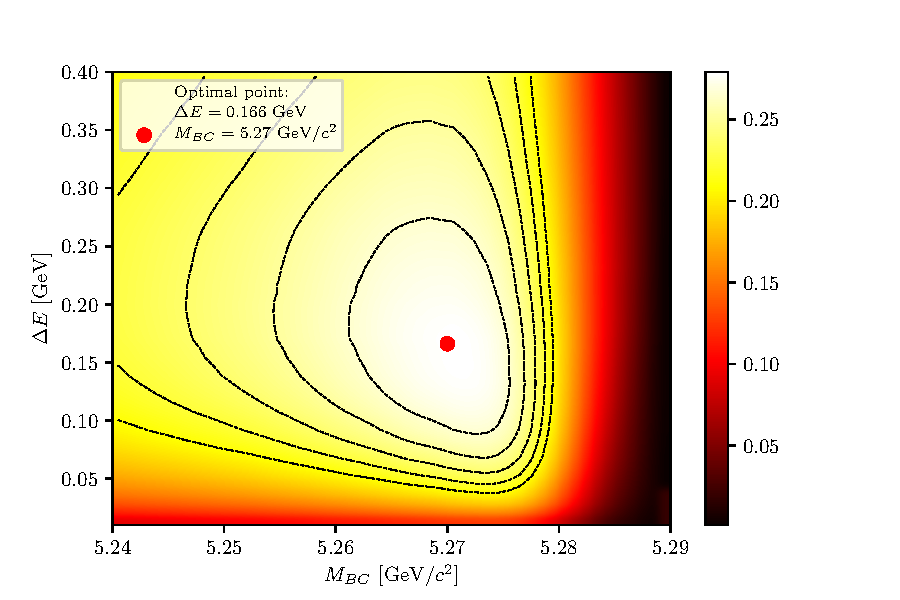
\includegraphics[width=\linewidth]{fig/sigWin}
\caption{2D $\mathrm{FOM}$ optimization of the signal region definition, where the signal in the optimization was represented by perfectly reconstructed candidates.}
\label{fig:sigwin}
\end{figure}

Lastly, we can tighten the cut on $m_{miss}^2$, which we intentionally left loose before the signal categorization. With the $\mathrm{FOM}$ optimization of perfectly reconstructed candidates inside the signal region, shown in Figure \ref{fig:missm2opt}, the optimal cut on $m_{miss}^2$ is 

\begin{itemize}
\item $\vert m_{miss}^2 \vert < 1.1\e{GeV}/c^2$.
\end{itemize}

\begin{figure}[H]
\centering
\captionsetup{width=0.8\linewidth}
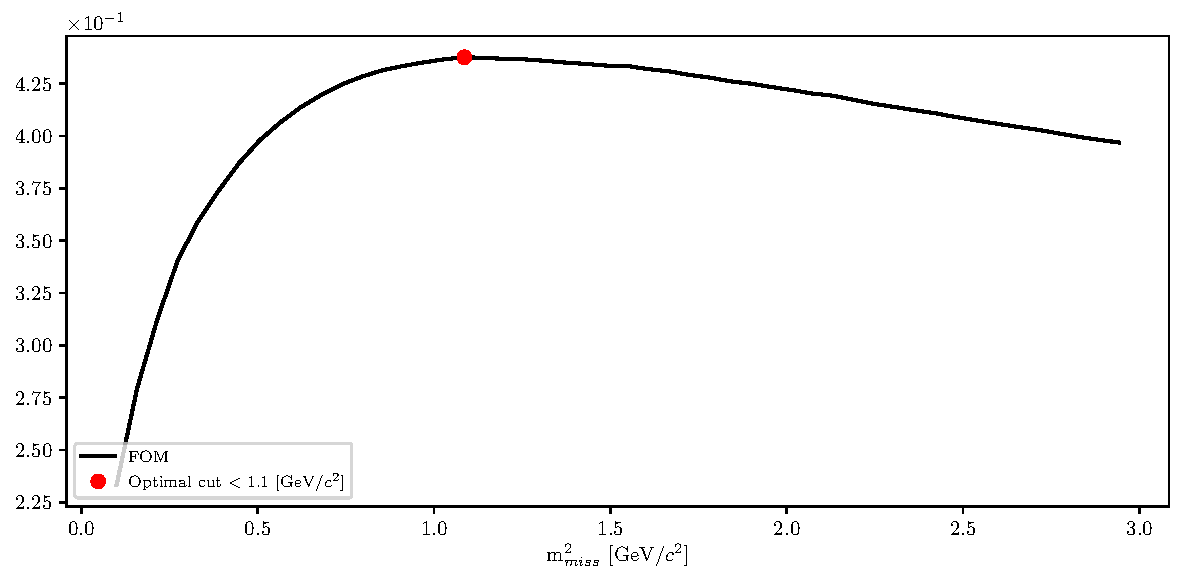
\includegraphics[width=\linewidth]{fig/missm2_opt}
\caption{$\mathrm{FOM}$ optimization of the optimal $m_{miss}^2$ cut in the signal region.}
\label{fig:missm2opt}
\end{figure}

\section{Selection summary}
\label{s:ss}
In this section one can find the summary of all selection cuts in the event reconstruction, from FSP particles up to the $B$ meson.

\begin{itemize}
\item FSP particles:
	\begin{itemize}
	\item Electrons: $\vert d_0 \vert < 0.1\e{cm},\,\vert z_0 \vert < 1,5\e{cm},\,p>0.6\e{GeV}/c,\\p_{CMS}\in[0.4,\,2.6]\e{GeV}/c,\,eID>0.9,$
    \item Muons: $\vert d_0 \vert < 0.1\e{cm},\,\vert z_0 \vert < 1,5\e{cm},\,p_{CMS}\in[0.6,\,2.6]\e{GeV}/c,\\\mu ID>0.97,$
    \item Kaons: $\vert d_0 \vert < 0.15\e{cm},\,\vert z_0 \vert < 1,5\e{cm},\,p_{CMS} < 2.5\e{GeV}/c,\\K/\pi~ID>0.6,\,K/p~ID>0.1,$
	\end{itemize}
\item $B$ meson candidates:
	\begin{itemize}
	\item Before ROE clean-up: $P(\chi^2,\,DOF) > 1\E{-3},\,\vert \cos \theta_{BY} \vert < 1,\,\vert m_{miss}^2 \vert < 7\e{GeV}/c^2,$
    \item After ROE clean-up: $\Delta E \in [-1.0,1.3]\e{GeV},\,M_{BC} \in [5.1,5.295]\e{GeV}/c^2,$
    \item After signal categorization: $q_{B^\pm}q_{B^\mp} = -1,\,BDT_{had.} > 0.51,\,\vert m_{miss}^2\vert<~1.1\e{GeV}/c^2.$
	\end{itemize}
\end{itemize}